\chapter{信頼性の効率的計算手法}\label{sec:proposed}
%\todo[inline]{TODO: 2章の文字の定義,ノード/節点/頂点,辺/弧を合わせる}

ADD \redout{を用いると},等価な節点の共有や冗長な節点の削除によって,
行列内の部分的に共通した情報を省略して表現できる.
\cyannout{しかし,行列はテンソル積によって急激に増加するため,
ADD による圧縮では不十分であると考えられる.
ADD の終端節点は,行列に含まれる値の種類数だけ存在するため,
行列のサイズが増加すれば,終端節点の数も増加しやすくなるからである.
終端\greenout{節}点の数が増加すると,それらを区別するための節点も増加し,
ADD のサイズは行列のサイズと相関する可能性がある.}

\cyannout{また,各ゲートに与えられる $p$ の値は,全て同じ値とは限らない.
既存手法では,全てのゲートで $p = 0.05$ 用いて\blueout{実験を行った}ため,
同じ部分行列が発生しやすく,ADD に適した状況となっている.
逆に,ゲートの出力が反転する確率として,いくつかの異なる値を設定した場合は,
節点の共有が発生しづらく,ADD \greenout{では対処できない}状況となることが予想される.}
\cyannout{大規模で多様な回路を評価するためには,}より効率的な計算方法が必要と\redout{考えられる}.

\section{評価式の変形による効率化手法}\label{sec:prop:deform}

%\paragraph{(${\it fidelity}({\bm v}, M, M_p) = {\bm v} \cdot {\bm s}$ について)}
既存手法では,行列 $M_p, M$ のサイズが問題となる.
そこで,提案手法ではこの行列を用いずに, $M_p .* M$ と等価な値を得る別のアプローチを検討する.

$M_p .* M$ は,正しい出力以外を 0 にする計算とみなすことができる.
$M_p .* M$ から,行ごとに 0 以外の要素を抜き出したベクトル ${\bm s}$ を用いると,
式~(\ref{eq:fidelity}) の値は,内積を用いて以下のように求めることができる.
\begin{eqnarray}
  {\it fidelity}({\bm v}, M, M_p) = {\bm v} \cdot {\bm s} \label{eq:deformed}
\end{eqnarray}

$M_p .* M$ が正しい出力を抜き出す処理と考えると, ${\bm s}$ の $\bm{i} + 1$ 番目の要素は,
2 進数として表したビット列 ${\bm i}$ を入力したときに正しい出力が得られる確率である.
\ref{sec:ptm-const} 節の例と同じ状況
(図~\ref{fig:exgate} の回路を,0.05 の確率で反転するゲートを用いて構成し,入力パターンが等確率で与えられる場合)
ならば, ${\bm s}$ は各要素が 0.9025 で要素数 8 のベクトルとなり,
行列を計算することなく, ${\bm v} \cdot {\bm s} = 0.9025$ が得られる.

\subsection{正しい出力が得られる確率の計算}

% 文字の定義
${\bm s}$ の各要素は,
組み合わせ回路 $C$ を無閉路有効グラフ $G_C = ({\it PI} \cup {\it PO} \cup V_C, E_C)$ として表し,
再帰的に計算することで求められる.
% 頂点について
${\it PI}, {\it PO}$ は,それぞれ外部入力と外部出力を表す頂点集合であり,
$V_C$ は,各ゲートの頂点集合である.
ゲート $g \in V_C$ が確率 $p$ で反転するとき, $err(g) = p$ とする.
% 辺について
ある頂点 $g'$ の出力が,頂点 $g$ に入力されている時,
2 個の頂点は入力される側から出力する側への有向辺 $(g, g') \in E_C$ で結ばれる.
また,頂点 $g$ のファンインを ${\it FI}(g)$,ファンアウトを ${\it FO}(g)$ で表す.
$g$ の入次数は $|{\it FI}(g)|$,出次数は $|{\it FO}(g)|$ となる.
$g \in {\it PI}$ の場合には $|{\it FI}(g)| = 0$ であり,
$g \in {\it PO}$ の場合には $|{\it FO}(g)| = 0$ である.

%\paragraph{(${\bm s}$ を計算するアルゴリズムについて)}
全ての外部出力が正しく出力されれば,正しい出力が得られている.
回路に ${\bm i}$ を入力した時のゲート $g$ が誤りとなる確率 ${\it fail}({\bm i}, g)$ とすると,
${\bm s}$ の各要素は以下のようになる.
\begin{eqnarray}
  {\bm s}({\bm i} + 1) = \prod_{g \in PO}(1 - {\it fail}({\bm i}, g)) \label{eq:allnofail}
\end{eqnarray}

${\bm i}$ を入力した時にゲート $g$ が誤りとなる確率 ${\it fail}({\bm i}, g)$ は,
ゲートのファンインで考えられる全てのエラーパターンに分けて考える.
エラーのパターンはビット列 ${\bm e}$ を用いて表す.
例えば, $|{\it FI}(g)| = 3$ のゲートに $(011)_2$ を入力し,
${\bm e} = (010)_2$ のエラーが発生した時,
ビット同士の XOR によって $(010)_2$ が入力されると考える.
全てのエラーパターン集合は,$\{0, 1\}^{|{\it FI}(g)|}$ で得ることができる.
\cyannout{すなわち,}頂点 $g$ でエラーパターン ${\bm e}$ が発生し,
\blueout{同時に反転の状態を出力が誤りとなるような}確率を求める.
\begin{eqnarray}
  {\it fail}({\bm i}, g) = {\displaystyle \sum_{{\bm e} \in \{0, 1\}^{|{\it FI}(g)|}}}
    O({\bm i}, g, {\bm e}) \times {\it toFail}({\bm i}, g, {\bm e}) \label{eq:fail}
\end{eqnarray}
ただし,$g \in {\it PI}$ の時,反転が発生することはないので,
\begin{eqnarray}
  {\it fail}({\bm i}, g) = 0
\end{eqnarray}
とする.

エラーパターン ${\bm e}$ の生起確率は,前段の頂点 $g'$ から計算される.
\begin{eqnarray}
  O({\bm i}, g, {\bm e}) = \prod_{\substack{g' \in {\it FI}(g),\\ e_{g'} \in {\bm e}}} \begin{cases}
    {\it fail}({\bm i}, g') & : e_{g'} = 1\\
    1 - {\it fail}({\bm i}, g') & : e_{g'} = 0
  \end{cases} \label{eq:occur}
\end{eqnarray}
${\bm e}$ の $i$ 番目の要素が 1 の時,$g$ の $i$ 番目の出力が誤って入力される確率が与えられる.
すなわち,式~(\ref{eq:occur}) は,全てのファンインが同時に ${\bm e}$ の表す状態になる確率を求めている.

${\it toFail}({\bm i}, g, {\bm e})$ は,ゲート $g$ が最終的に誤った出力となるように反転する確率である.
回路に ${\bm i}$ を入力した時のゲート $g$ の正しい出力を ${\it out}({\bm i}, g)$ とし,
${\bm i}$ を入力してエラーパターン ${\bm e}$ が発生した時のゲート $g$ の出力を
${\it act}({\bm i}, g, {\bm e})$ とする.
%これらの結果を比較して,このゲートが反転するべきかどうかを判断し,\blueout{式~(\ref{eq:to_fail})} のように計算する.
これらの結果から,\blueout{このゲートが誤った出力となるためには,}反転\blueout{した状態になる}べきかどうかを判断し,\blueout{式~(\ref{eq:to_fail})} のように計算する.
\begin{eqnarray}
  {\it toFail}({\bm i}, g, {\bm e}) = \begin{cases}
    {\it err}(g) & : {\it out}({\bm i}, g) = {\it act}({\bm i}, g, {\bm e})\\
    1 - {\it err}(g) & : {\it out}({\bm i}, g) \neq {\it act}({\bm i}, g, {\bm e})
  \end{cases} \label{eq:to_fail}
\end{eqnarray}
入力の誤りに関わらず,論理マスクの影響によって正しい出力が得られる場合,
ゲート $g$ は\blueout{出力が誤りになるように}反転しなくてはならない.
一方,入力の誤りが出力に影響を与え,最終的に誤った出力となる場合には,
ゲート $g$ はその誤った出力を次のゲートへ入力する必要がある.
例えば,\greenout{2 入力の AND ゲート $g$ が存在する回路の外部入力に \blueout{${\it bin}({\bm i})$} を与えた結果,
\cyannout{回路内に存在する} AND ゲート $g$ に $(00)_2$ が入力された}とする.
このとき,正しいゲートの出力は ${\it out}({\bm i}, g) = 0$ となる.
ゲート $g$ の出力が本来とは異なるようになるためには,
$bin({\bm e}) = (11)_2$ の場合に反転せず,それ以外では反転しなくてはな\blueout{ら}ない.

式~(\ref{eq:fail}) の $O({\bm i}, g, {\bm e}) \times {\it toFail}({\bm i}, g, {\bm e})$ は,
エラーパターン ${\bm e}$ が発生し,かつ,
そのエラーパターンの時に最終的なゲート $g$ の出力が正しい値から反転する確率を求めている.
全てのエラーパターンについて場合分けを行い,それぞれの状態についての確率の和\greenout{を求めることで},
そのゲートの出力が誤りとなる確率\greenout{を得る}.

%\paragraph{(擬似コードを用いた議論)}
\begin{algorithm}[tbp]
  \caption{{\bf fail}: 与えられたノードの出力が反転する確率を求める}
%  \caption{{\bf fail}: Calculating a probability that gate $g$ outputs an incorrect galue}
  \label{alg:failprob}
  \begin{algorithmic}[1]
    \REQUIRE ${\it g}$: 出力のエラー率を求めるノード
%    \REQUIRE ${\it g}$: the gate for the calculation
    \IF{$g \in PI$}
      \RETURN 0
    \ENDIF
    \IF{$g$ はすでに計算済み}
      \RETURN ${\it fail\_cache}[g]$
    \ENDIF
    \STATE ${\it res} = 0$
    \FORALL{${\bm e} \in \{0, 1\}^{|{\it FI}(g)|}$}
      \STATE $O \leftarrow 1$
      \FORALL{$g' \in {\it FI}(g), e_{g'} \in {\bm e}$}
        \IF{$e_{g'} = 1$}
          \STATE $O \leftarrow O \times {\it fail}(g')$
        \ELSE
          \STATE $O \leftarrow O \times (1 - {\it fail}(g'))$
        \ENDIF
      \ENDFOR
      \STATE ${\it res} \leftarrow {\it res} + O \times {\it toFail}(g, {\bm e})$
    \ENDFOR
    \STATE ${\it fail\_cache}[g] \leftarrow res$
    \RETURN ${\it res}$
  \end{algorithmic}
\end{algorithm}
実際の計算では,各入力を終端ノードに設定してから Algorithm~\ref{alg:failprob} のように再帰的に計算を行う.
9-16行目が式~\ref{eq:occur} の計算に相当する.
${\it toFail}$ の計算に用いる ${\it out}$ の値は,入力の設定時に事前に計算することができる.
また,${\it act}$ の値は, ${\it out}$ と ${\bm e}$ を用いて計算できる.
この計算は,全ての出力線から開始しなくてはならない.

関数 ${\it fail}$ の結果は,入力パターンとノードの組に対して一意に定まるので,
一度求めた結果は再利用することができる.
具体的には,Algorithm~\ref{alg:failprob} に加えて, $g$ に対する値を計算していないか調べ,
存在すればその値を返すような処理行なえばよい.
また,入力パターンを変更するごとに計算結果を\cyannout{消去}している.
したがって,1 個の入力パターンに対しては,
\greenout{式~(\ref{eq:allnofail})} のように $|PO|$ 回だけ再帰を開始しなくてはならないが,
パターンを設定してから\greenout{ 2 個}目以降の外部出力に対する結果は,
過去に計算した値を利用できる場合があるため比較的少ない時間で求められると期待できる.

%\paragraph{(ゲートの分割)}
Algorithm~\ref{alg:failprob} の 8-18 行目のループは,
一度の呼び出しで $2^{|FI(g)|} \times |FI(g)|$ 回実行される可能性がある.
そこで,4 入力以上を持つゲート ($|FI(g)| \geq 4$) は,2 入力のゲートに分割して計算しなくてはならない.
このとき,元のゲートの出力が反転する確率と,分割後の最終段のゲートの出力が反転する確率は等しく,
それ以外は反転を発生しないゲートとする.
このように回路を変形させることで,$2^{|FI(g)|} \times |FI(g)|$ 回のループを,
$2^3$ 回のループを含んだ $|FI(g)| - 1$ 回の関数呼び出しに置き換えることができる.

\subsection{異なる入力間での計算結果の再利用}\label{sec:prop:deform:reuse}

%The calculation can also start from the nodes corresponding the primary inputs
%by the topological order instead of the above method.
関数 ${\it fail}$ は,外部入力側のノードからトポロジカル順に計算することもできる.
%It is enough to calculate the output of a gate whose input values are changed
%since the probability of flipping depends on the input values.
このとき,最終的に出力が誤る確率は入力に依存するため,
変化した入力に依存したノードのみを更新すれば十分である.
\begin{figure}[tbp]
  \begin{center}
    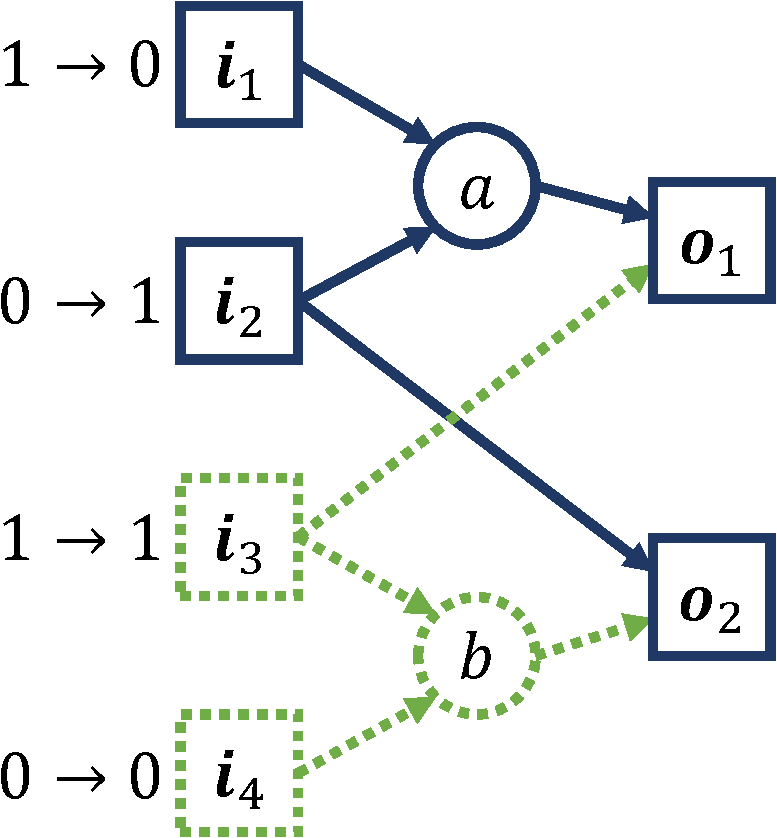
\includegraphics[width=64mm,clip]{img/update_graph.pdf}
  \end{center}
%\caption{4入力2出力の回路の例と再計算}
%  \caption{Recalculation when the input pattern is changed
%  where a circuit which has four primary inputs, two primary outputs and two gates}
  \caption{4入力2出力の回路ににおける入力パターンが変更した際の再計算}
\label{fig:update_graph}
\end{figure}
%Fig.~\ref{fig:update_graph} shows the recomputation in the nodes depending on the changed inputs.
図~\ref{fig:update_graph} は入力が変化した際に,再計算を行うノードを示している.
%In this example, the calculation starts from nodes ${\bm i}_1$ and ${\bm i}_2$
%and updates node $a$, ${\bm o}_1$ and ${\bm o}_2$ in order.
この例では,入力が変化した ${\bm i}_1, {\bm i}_2$ から開始して,$a, {\bm o}_1, {\bm o}_2$ の順に更新する.
%We do not have to calculate the probability on node $b$
%since the dependent nodes: both ${\bm i}_3$ and ${\bm i}_4$, do not change their values.
${\bm i}_3, {\bm i}_4$ の入力は変化しないため,これらのみに依存するノード $b$ は更新する必要がない.
このようにすると,変化した入力に依存するノードのみを再計算できる.

%\paragraph{(グレイコードを用いる)}
計算順序の変更に加えて,入力パターンの割り当てにグレイコードを用いることで,
さらに計算時間を短縮できる.
%In addition to the reverse of the calculation order, assignment of the input pattern by Gray Code saves time.
%Gray Code can enumerate all the input patterns such that the two adjacent input patterns differs at only one bit.
%Then we can reduce the started nodes to recalculate.
グレイコードは,1ビットのみを変更させながら,全ての入力パターンを列挙できるため,
再計算が開始されるノードを減らすことができるからである.
%When we generate the input patterns by the simple ascending order of binary number,
%there is a case that multiple inputs are changed between two input patterns.
入力パターンを単純な2進数を用いて0から順番に割り当てると,
全てのビットが変化してしまうケースが存在する.
%e.g. $(011)_2 \to (100)_2$ (We need start from the three nodes since the assignment of the three inputs are different).
例えば,$(011)_2 \to (100)_2$ のような変化は,3 箇所のが変化し,3 個のノードから開始しなくてはならない.
%Therefore, by using Gray Code, we can start from the single node at all times after the calculation of the first pattern.
それに対し,グレイコードを用いると,
2つ目以降の入力パターンについては,常に 1 個のノードから再計算をするだけで十分となる.

\subsection{正しい確率が得られないケース}

\begin{figure}[tbp]
  \begin{center}
    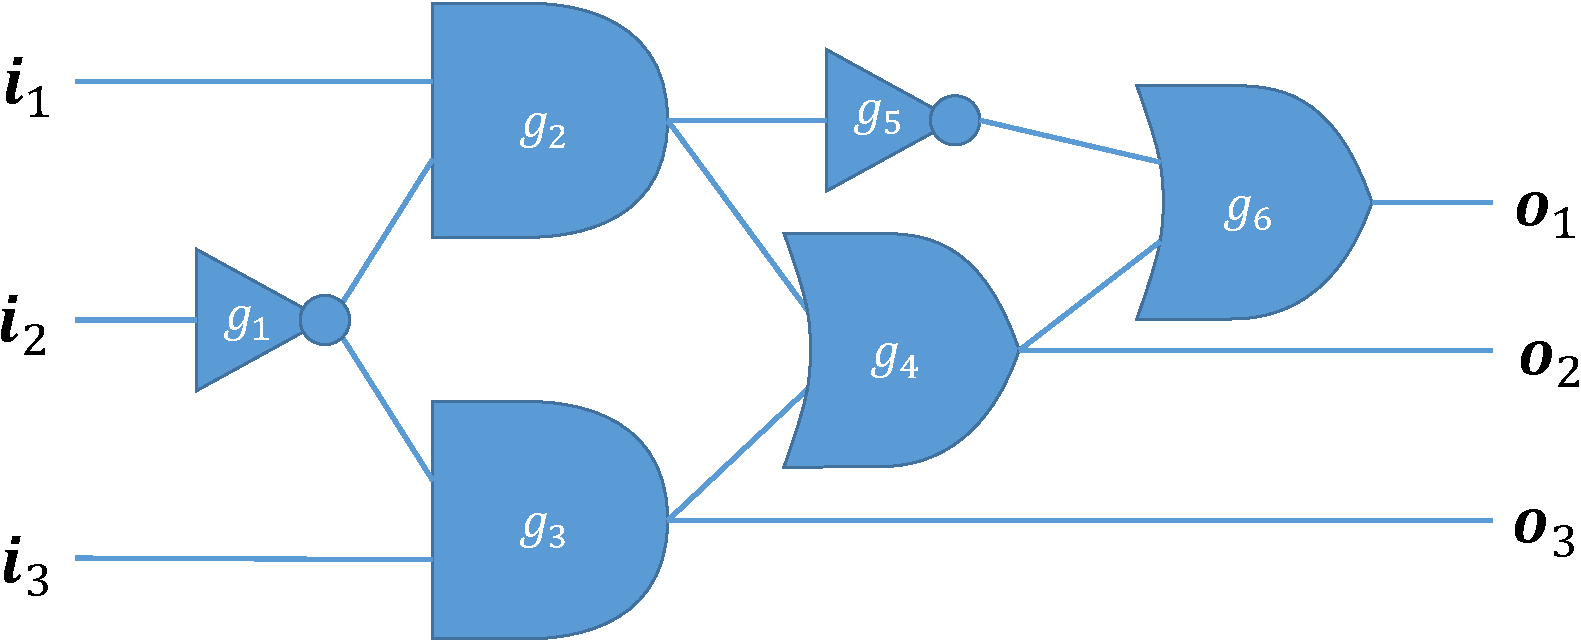
\includegraphics[height=50mm,clip]{img/join.pdf}
  \end{center}
  \caption{2 箇所の再収斂によって正確な結果が得られない例}
  \label{fig:join}
\end{figure}
%Our method may calculate inaccurate probabilities
%if the circuit contains fan-out points which may reconverge later.
ここまで提案してきた手法では,回路に再\greenout{収}斂を含むケースに対して正確な結果を得ることができない.
%When we use the method just as it is, the result contains a contradicted suppositions
%that the different soft-error occurrence at the same gate between inputs.
回路に再\greenout{収}斂が含まれている場合,計算結果には,
同一のゲートに対して異なるソフトエラー発生の状態を仮定した計算が含まれてしまうからである.
%TODO グラフの分割と合成
%In the case of Fig~\ref{fig:join}, the inputs of gate $g_4$ branch from the outputs of gate $g_1$.
例えば,図~\ref{fig:join} のようなケースにおいて,$g_1$ から分岐した出力は $g_4$ へ 2 通りの経路から入力される.
%Then the calculation at gate $g_2$ suppose that the error occur or does not occur,
%この時,ゲート $g_4$ の結果は,ゲート $g_1$ でエラーが起きた場合と起きない場合の両方の仮定を用いている.
この時,ゲート $g_4$ の結果は,\redout{ゲート $g_1$ でエラーが起きた場合と起きない場合の矛盾した仮定を用いているため,
ここまで述べてきた手法では,誤った値を計算していることになる}.
%and the calculation at gate $g_3$ also supposes that.
また,ゲート $g_3$ の結果も両方の仮定を用いている.
%In the calculation at gate $g_4$, even though the calculation of $g_2$ supposes that the error occur,
したがって,$g_4$ での計算は,$g_2$ の計算で $g_1$ にエラーが発生しないと仮定したにもかかわらず,
%the calculation of $g_4$ contains the cases supposing that the error does not occur.
$g_4$ の計算で $g_1$ にエラーが発生すると仮定して計算した場合を含んでしまう.
%The calculation at gate $g_5$ also contains supposition.
ゲート $g_2$ の分岐でも,同様に\redout{矛盾した仮定を用いて計算してしまう}.
%However, it should be noted that this kind of errors would not be so problematic
%in many cases as our experimental results show in the next section.
%しかしながら,少なくとも本研究で行った実験ではこのようなケースはそれほど大きな誤差を引き起こさない.

\section{数式処理による計算手法}\label{sec:prop:exp}

% 概要

関数 ${\it fail}$ の計算において誤った結果となってしまうのは,
同一のゲートについて,実際には発生しない状態を仮定をしてしまうからである.
そこで,再\greenout{収}斂の元となるファンアウト・ポイントに対し変数を定義することで,
この状態の計算を修正することを考える.

\subsection{補正ルールの検討}

\begin{figure}[tbp]
  \begin{center}
    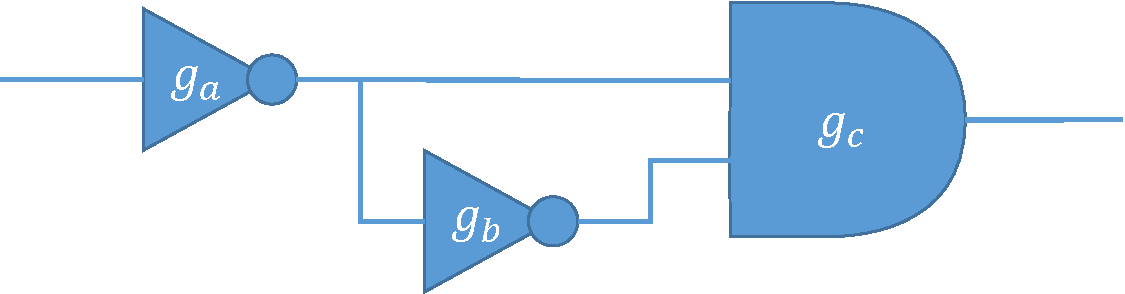
\includegraphics[height=25mm,clip]{img/min-reconv.pdf}
  \end{center}
  \caption{再収斂が 1 箇所存在するケース}
  \label{fig:min-reconv}
\end{figure}
再収斂が問題となるケースとして,図~\ref{fig:min-reconv} のような回路を考える.
ここで,ゲート $g_a$ の出力が異なる状態を仮定してしまうのが問題である.
そこで,ゲート $g_a$ の出力が最終的に 1 となる確率を $P(g_a)$ とおく.
他のゲートについて出力が 1 となる確率を求めると,以下のようになる.
\begin{eqnarray}
P(g_b) &=& P(g_a) {\it err}(g_b) + (1 - P(g_a)) (1 - {\it err}(g_b)) \nonumber \\
P(g_c) &=& P(g_a \cap g_b) (1 - {\it err}(g_c)) + (1 - P(g_a \cap g_b)) {\it err}(g_c) \nonumber
\end{eqnarray}
$g_b$ は $g_a$ に依存して\redout{いるため},
\redout{ゲート $g_a, g_b$ の出力}が同時に 1 になる確率は,$P(g_a) P(g_b)$ では正しく計算出来ない.
\[ P(g_a) P(g_b) = P(g_a)^2 {\it err}(g_b) + P(g_a) (1 - P(g_a)) (1 - {\it err}(g_b)) \]
\redout{ゲート $g_a, g_b$ の出力}が同時に 1 になる正しい確率は,
\[ P(g_a \cap g_b) = P(g_a) {\it err}(g_b) \]
である.
そこで,3 種類の状況について,以下のように補正する.
\begin{description}
  \item[補正ルール 1] $P(g_i)^2 \rightarrow P(g_i)$
  \item[補正ルール 2] $(1 - P(g_i))^2 \rightarrow (1 - P(g_i))$
  \item[補正ルール 3] $P(g_i) (1 - P(g_i)) \rightarrow 0$
\end{description}
{\bf 補正ルール 2} は,出力が 0 となる場合について {\bf 補正ルール 1} と同様に補正することを示している.
また,同一のゲートであるため,反転が発生する状態と発生しない状態は同時に起こり得ない.
そこで {\bf 補正ルール 3} のように 0 に置き換える.

ここで,\redout{{\bf 補正ルール2},{\bf 補正ルール3} の左辺を展開し,
{\bf 補正ルール1} を}適用した場合,
\begin{description}
  \item[補正ルール 2] $(1 - P(g_i))^2 = 1 - 2 P(g_i) + P(g_i)^2 \rightarrow (1 - P(g_i))$
  \item[補正ルール 3] $P(g_i) (1 - P(g_i)) = P(g_i) - P(g_i)^2 \rightarrow 0$
\end{description}
となるため,{\bf 補正ルール1} のみを適用するだけで十分であるということがわかる.

\subsection{補正ルールを考慮した数式処理システム}

\redout{{\bf 補正ルール1} を適用するため}には,計算途中の情報を数式として保持する方法が考えられる.
再\greenout{収}斂されるノードでは,$P(g_i)$ を区別できないため,
\redout{単に数値として確率を表現している場合に}は,補正ルールを適用することができないからである.
そこで,補正ルールを考慮した数式処理システムを構築する.

$P(g_i)$ を記号として保持し,乗算の演算を行う際に補正ルールを適用させながら数式を処理する.
この時,$P(g_i)^2 \rightarrow P(g_i)$ のルールから,
2 以上の整数を $t$ として $P(g_i)^t \rightarrow P(g_i)$ が考えられる.
%したがって,現れる数式の項は 2 以上の指数を考える必要が無く,係数と変数の集合だけを管理すればよい.
\redout{したがって,現れる数式の各変数に関して 2 次以上の項}を考える必要が無く,係数と変数の集合だけを管理すればよい.

% 方針と項の表現方法
のちに再収斂が発生するファンアウト・ポイントの集合を $R$ で表す.
すなわち,$g \in R$ ならば,$P(g)$ は数式中で変数として表現しなくてはならない.
2 以上の指数を考えない場合,係数と変数の組み合わせの組で項を表し,
その集合によって以下のように数式を表現することができる.
\begin{eqnarray}
  F_e = \{ ({\it coeff}, {\it vars}) | {\it vars} \in \{0, 1\}^{|R|}, {\it coeff} = F({\it vars}) \}
\end{eqnarray}
例えば,$R = \{a, b\}$ において,$F(a, b) = 3ab + b$ を表す場合を考えると,
\[ F(0, 0) = F(1, 0) = 0 \]
\[ F(0, 1) = 1, F(1, 1) = 3 \]
\[ F_e = \{ (0, (0, 0)), (1, (0, 1)), (0, (1, 0)), (3, (1, 1)) \} \]
となる.
提案手法に必要な演算は,加減算と乗算である.
上記のように数式を表現した場合,これらの演算は集合の操作によって実現することができる.

\begin{algorithm}[tbp]
  \caption{{\bf operator} $+$: 数式同士の加算}
  \label{alg:add}
  \begin{algorithmic}[1]
    \REQUIRE $F_e, G_e$: 加算を行う多項式を表す集合
      \STATE ${\it result} \leftarrow \COMMENT{ハッシュテーブル} \varnothing$
      \FORALL{$({\it coeff}, {\it vars}) \in F_e \cup G_e$}
        \STATE ${\it result}[{\it vars}] \leftarrow ({\it result}[{\it vars}] {\mbox ~or~ } 0) + {\it coeff}$
      \ENDFOR
    \RETURN ${\it result}$
  \end{algorithmic}
\end{algorithm}
加算は,項の変数の組み合わせごとに分類し,係数の合計を求めれば良い.
加算のアルゴリズムを Algorithm~\ref{alg:add} に示す.
このアルゴリズムによって,${\it vars}$ と ${\it coeff}$ の対応が得られるので,
そこから $({\it coeff}, {\it vars})$ の集合を生成することができる.
同様のアルゴリズムを用いて,減算も実現することができる.

\begin{algorithm}[tbp]
  \caption{{\bf operator} $\times$: 数式同士の {\bf 補正ルール1} を適用した乗算}
  \label{alg:times}
  \begin{algorithmic}[1]
    \REQUIRE $F_e, G_e$: 乗算を行う多項式を表す集合
      \STATE ${\it result} \leftarrow \COMMENT{ハッシュテーブル} \varnothing$
      \FORALL{$(t_F, t_G) \in F_e \times G_e$}
        \STATE ${\it vars} \leftarrow (t_F.{\it vars} \; | \; t_G.{\it vars})$
        \STATE ${\it coeff} \leftarrow (t_F.{\it coeff} \; | \; t_G.{\it coeff})$
        \STATE ${\it result}[{\it vars}] \leftarrow ({\it result}[{\it vars}] {\mbox ~or~ } 0) + {\it coeff}$
      \ENDFOR
    \RETURN ${\it result}$
  \end{algorithmic}
\end{algorithm}
乗算は, 2 個の数式に含まれる項について乗算を行い,加算と同様に分類する.
乗算のアルゴリズムを Algorithm~\ref{alg:times} に示す.
ここで, `$|$' は要素同士の OR を表す.
項同士の乗算は,係数部分と変数部分に分けて行われ,
変数部分については,要素同士の OR で計算できる.

Algorithm~\ref{alg:add},~\ref{alg:times} で示された通り,
数式の演算にはハッシュテーブルが必要となる.
したがって,${\it vars}$ についてはハッシュ値を計算しなくてはならない.
${\it vars}$ がビット列で表されている場合には,ビット数に比例する時間でハッシュ値を計算できる.
あるいは,変数の組み合わせを,単一の組み合わせのみを含む特殊な
Zero-suppressed BDD (ZDD)~\cite{zdd-app} として表すこともできる.
同一の組み合わせかどうかは ZDD の節点番号を用いて判別でき,
ハッシュ値もこの節点番号を用いれば良い.
要素同士の OR は, ZDD の Join 演算~\cite{knuth2014art} を用いて実現できる.

%\todo[inline]{今後の課題に「係数を開始側に置くか終端側に置くか」を追加}

\subsection{数式の生成}

% アルゴリズムの書き換え

\begin{algorithm}[tbp]
  \caption{$P(g)$: 与えられたノードの出力が 1 になる確率についての数式を求める}
%  \caption{{\bf fail}: Calculating a probability that gate $g$ outputs an incorrect galue}
  \label{alg:oneex}
  \begin{algorithmic}[1]
    \REQUIRE ${\it g}$: 出力のエラー率を求めるノード
%    \REQUIRE ${\it g}$: the gate for the calculation
    \IF{$g \in PI$ もしくは,$g$ はファンアウト・ポイント}
      \RETURN\COMMENT{ 記号としての } $P(g)$
    \ENDIF
    \IF{$g$ はすでに計算済み}
      \RETURN ${\it one\_ex\_cache}[g]$
    \ENDIF
    \STATE ${\it res} = 0$
    \FORALL{${\bm b} \in \{0, 1\}^{|{\it FI}(g)|}$}
      \STATE $O \leftarrow 1$
      \FORALL{$g' \in {\it FI}(g), b_{g'} \in {\bm b}$}
        \IF{$b_{g'} = 1$}
          \STATE $O \leftarrow O \times P(g')$ \COMMENT{ ルールを適用した数式としての計算 }
        \ELSE
          \STATE $O \leftarrow O \times (1 - P(g'))$ \COMMENT{ ルールを適用した数式としての計算 }
        \ENDIF
      \ENDFOR
      \STATE ${\it res} \leftarrow {\it res} + O \times {\it toBeOne}(g, {\bm b})$ \COMMENT{ ルールを適用した数式としての計算 }
    \ENDFOR
    \STATE ${\it one\_ex\_cache}[g] \leftarrow res$
    \RETURN ${\it res}$
  \end{algorithmic}
\end{algorithm}
数式は,後に再収斂するファンアウト・ポイントで分割し,各部分回路ごとに生成する.
各ゲートの出力が 1 になる確率を計算する数式を生成するアルゴリズムは Algorithm~\ref{alg:oneex} のようになる.
${\it fail}$ の計算と同様,入力パターンの生起確\greenout{率}と,その入力の際に 1 になる確率によって計算できる.
${\it toBeOne}$ はゲートにビット列 ${\it bin}({\bm b})$ を入力した際に,ゲート\redout{の出力}が 1 になるための確率を返す.
この関数は式~(\ref{eq:to_be_one}) の様に計算できる.
\begin{eqnarray}
  {\it toBeOne}(g, {\bm b}) = \begin{cases}
    {\it err}(g) & : {\it logic}(g, {\bm b}) = 0 \\
    1 - {\it err}(g) & : {\it logic}(g, {\bm b}) = 1
  \end{cases} \label{eq:to_be_one}
\end{eqnarray}
このとき,${\it logic}(g, {\bm b})$ は,ゲート $g$ にビット列 ${\bm b}$ を入力した際の出力を返す.

\cyannout{ある入力について構成された数式は,他の入力においても再利用できる.
これは,入力を 0 から 1 に変えることと,外部入力が反転する確率が 0 から 1 になることが等価であるからである.
そこで,のちに再収斂が発生するファンアウト・ポイントの集合 $R$ に加え,
外部入力 ${\it PI}$ に含まれるノードについても変数として扱う.
したがって,$P(g), g \in \{ R \cup {\it PI} \}$ を変数とした数式が生成され,
各外部入力が 1 になる確率を与えることで,外部入力の信頼性を計算できる.}

${\bm s}$ の導出は,外部入力からトポロジカル順に,$P(g)$ へ値を割り当てることで求めることができる.
$P(g)$ は,1 となる確率であるから,$g_i \in PI$ の場合は,
1 を入力する場合は $P(g_i) = 1$,0 を入力する場合は $P(g_i) = 0$ とすればよい.
Algorithm~\ref{alg:oneex} によって,部分回路の出力が 1 となる確率を得ることができるので,
その結果を,対応するファンアウト・ポイントの変数へ代入することで,さらに別な部分回路の出力について計算できる.
全ての部分回路について計算すると,外部出力が 1 となる確率を得ることができ,
別に計算した ${\it out}({\bm i}, v)$ の結果と合わせて,
正しい出力が得られる確率 ${\bm s}({\bm i} + 1)$ を得る.

\begin{figure}[tbp]
  \begin{center}
    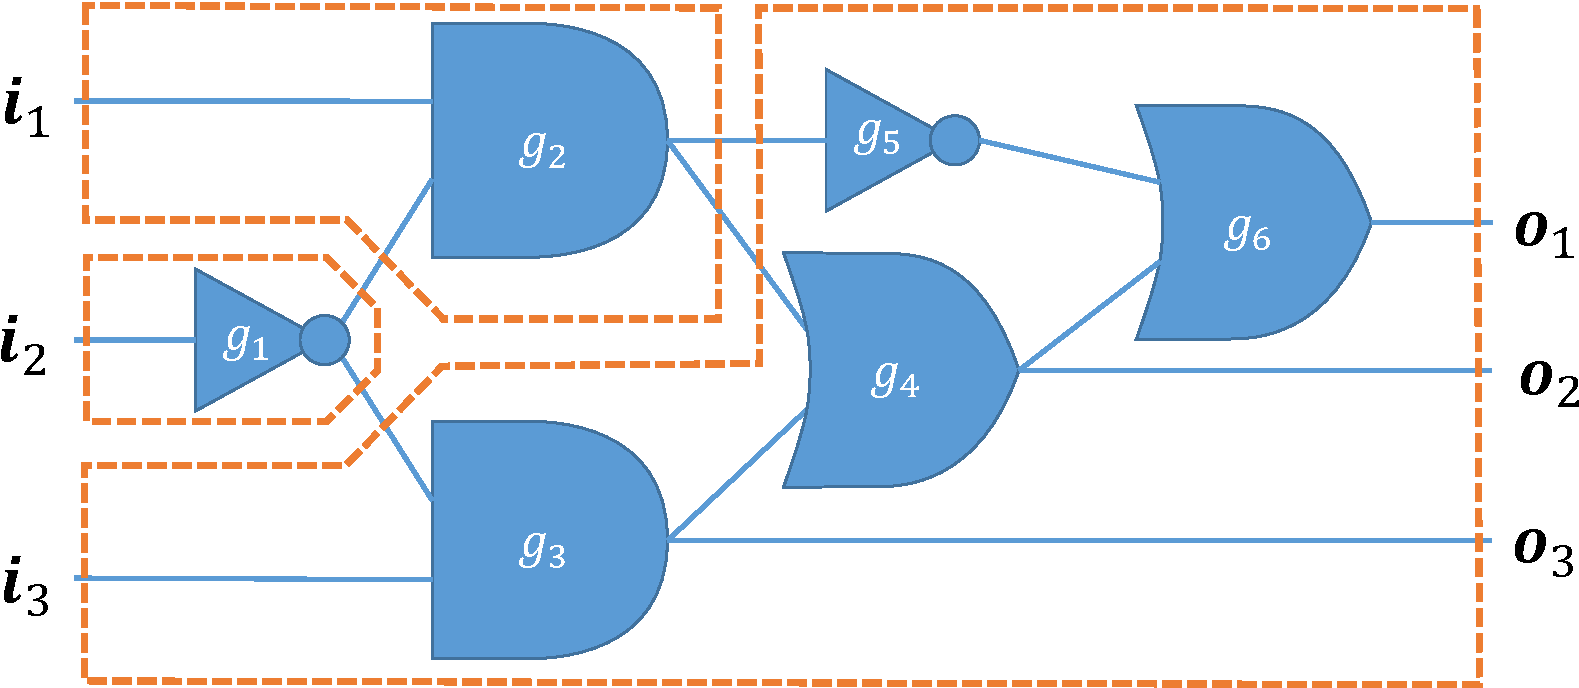
\includegraphics[height=60mm,clip]{img/fan-out-div.pdf}
  \end{center}
  \caption{図~\ref{fig:join} の回路を分割する例}
  \label{fig:fan-out-div}
\end{figure}
例えば,図~\ref{fig:join} の回路は,図~\ref{fig:fan-out-div} のように分割する.
$P({\bm i_2})$ を用いて $P(g_1)$ を表し,$P({\bm i_1}), P(g_1)$ を用いて $P(g_2)$ を表し,
$P(g_1), P(g_2), P({\bm i_3})$ を用いて $P({\bm o_1}), P({\bm o_2}), P({\bm o_3})$ を表す.
この時,数式は {\bf 補正ルール1} に従って生成される.
${\bm s}(0)$ の場合は,$P({\bm i_1}) = P({\bm i_2}) = P({\bm i_3}) = 0$ として計算し,
それ以外の要素についても同様に計算することで,正確な結果を求めることができる.
